\documentclass{article}
\usepackage[T1]{fontenc}
\usepackage{lmodern}
\usepackage{graphicx}
\usepackage{amsmath,amssymb}
\usepackage[a4paper,margin=2cm]{geometry}
\usepackage[absolute,overlay]{textpos}
\setlength{\TPHorizModule}{1mm}
\setlength{\TPVertModule}{1mm}
\usepackage[indonesian]{babel}
\usepackage{hyperref}
\setlength{\emergencystretch}{2em}
% unit: Halaman 15

\begin{document}

% === Halaman 15 (llm) ===

ATM mengenkripsi PIN dengan kunci $k$ lalu mengirim cipherteks ke komputer di bank

\[ \text{Cipher}(k, PIN) \]

\vspace{20mm}

Kriptanalis ke-1 mengubah PIN lalu memasukkan PIN tsb ke ATM

\vspace{20mm}

Kriptanalis ke-2 menyadap cipherteks dan mempelajarinya untuk mendeduksi kunci $k$

\vspace{10mm}

\begin{center}
\Large \textit{Chosen-plaintext attack}
\end{center}

% deskripsi: Diagram ilustrasi Chosen-plaintext attack yang menunjukkan interaksi antara pengguna/kriptanalis, mesin ATM, bank, dan penyadap (kriptanalis kedua).
% bbox normalisasi: [0.1400, 0.2000, 0.9000, 0.7200]
\begin{textblock*}{159.60mm}(29.40mm,59.40mm)
\noindent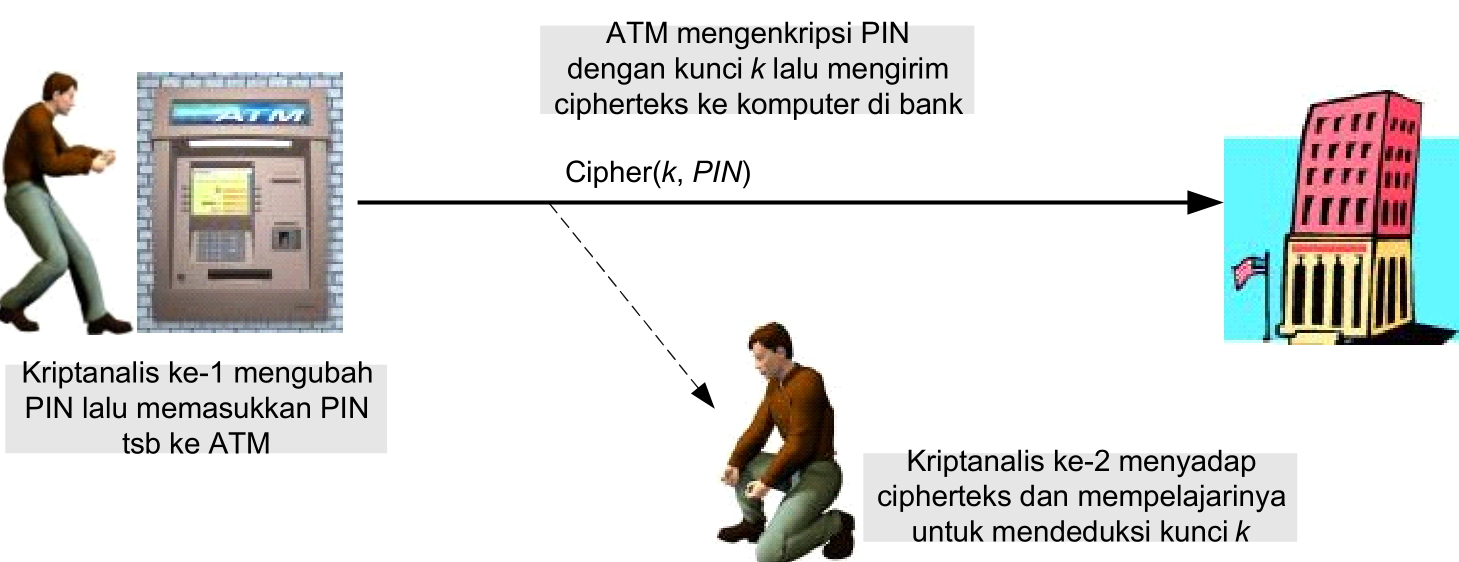
\includegraphics[width=159.60mm,height=154.44mm]{../../images/llm/page_015_img_01.png}%
\end{textblock*}

\end{document}
